\newpage
\chapter{Results}

These results were computed using the \verb+julia test_all.jl+ script which runs the two Cbc and GLPK solvers on all instances (30 easy instances and 10 hard instances) and writes the minimized objective function value and performance result of each instance in respective files in the \verb+results+ folder. For a better readability, we chose to make a separate result table per solver.

We did not consider the results for P3 alone because it is not supposed to be run on the whole index set $T$.
Also, it remains considerably slow on hard instances.

\section{Cbc}

\begin{table*}[h!]\centering
\ra{1.3}
\begin{tabular}{@{}rrrcrrcrr@{}}\toprule
& \multicolumn{2}{c}{P1} & \phantom{abc} & \multicolumn{2}{c}{P3 BIN} & \phantom{abc} & \multicolumn{2}{c}{P3 DB3}\\
\cmidrule{2-3} \cmidrule{5-6} \cmidrule{8-9}
& Obj & Time(s) & & Obj & Time(s) & & Obj & Time(s)\\ \midrule
instance10\_1\_1.dat & 75 & 2.422 & & 75 & 0.899 & & 75 & 0.214 \\
instance10\_1\_2.dat & 72 & 0.077 & & 72 & 0.018 & & 72 & 0.020 \\
instance10\_1\_3.dat & 85 & 0.080 & & 85 & 0.013 & & 85 & 0.018 \\
instance10\_1\_4.dat & 72 & 0.090 & & 72 & 0.014 & & 72 & 0.023 \\
instance10\_1\_5.dat & 70 & 0.089 & & 70 & 0.015 & & 70 & 0.020 \\
instance10\_2\_1.dat & 34 & 0.184 & & 34 & 0.019 & & 34 & 0.024 \\
instance10\_2\_2.dat & 43 & 0.123 & & 43 & 0.113 & & 43 & 0.050 \\
instance10\_2\_3.dat & 46 & 0.183 & & 46 & 0.039 & & 46 & 0.031 \\
instance10\_2\_4.dat & 42 & 0.103 & & 42 & 0.073 & & 42 & 0.032 \\
instance10\_2\_5.dat & 29 & 0.166 & & 29 & 0.040 & & 29 & 0.040 \\
instance10\_5\_1.dat & 9 & 0.132 & & 9 & 0.200 & & 9 & 0.015 \\
instance10\_5\_2.dat & 10 & 0.111 & & 10 & 0.100 & & 10 & 0.016 \\
instance10\_5\_3.dat & 9 & 0.100 & & 9 & 0.103 & & 9 & 0.030 \\
instance10\_5\_4.dat & 9 & 0.088 & & 9 & 0.132 & & 9 & 0.021 \\
instance10\_5\_5.dat & 11 & 0.097 & & 11 & 0.104 & & 11 & 0.015 \\
instance20\_2\_1.dat & 39 & 0.375 & & 39 & 0.293 & & 39 & 0.106 \\
instance20\_2\_2.dat & 53 & 1.570 & & 53 & 1.249 & & 53 & 0.136 \\
instance20\_2\_3.dat & 55 & 1.312 & & 55 & 0.365 & & 55 & 0.121 \\
instance20\_2\_4.dat & 51 & 1.163 & & 51 & 0.163 & & 51 & 0.166 \\
instance20\_2\_5.dat & 55 & 1.333 & & 55 & 0.920 & & 55 & 0.104 \\
instance20\_4\_1.dat & 21 & 0.260 & & 21 & 0.311 & & 21 & 0.043 \\
instance20\_4\_2.dat & 24 & 0.327 & & 24 & 0.061 & & 24 & 0.053 \\
instance20\_4\_3.dat & 23 & 0.261 & & 23 & 0.067 & & 23 & 0.088 \\
instance20\_4\_4.dat & 17 & 0.448 & & 17 & 0.074 & & 17 & 0.096 \\
instance20\_4\_5.dat & 22 & 0.342 & & 22 & 0.524 & & 22 & 0.080 \\
\end{tabular}
\end{table*}
\newpage
\begin{table*}[h!]\centering
\ra{1.3}
\begin{tabular}{@{}rrrcrrcrr@{}}\toprule
& \multicolumn{2}{c}{P1} & \phantom{abc} & \multicolumn{2}{c}{P3 BIN} & \phantom{abc} & \multicolumn{2}{c}{P3 DB3}\\
\cmidrule{2-3} \cmidrule{5-6} \cmidrule{8-9}
& Obj & Time(s) & & Obj & Time(s) & & Obj & Time(s)\\ \midrule
instance20\_10\_1.dat & 3 & 0.046 & & 3 & 0.863 & & 3 & 0.057 \\
instance20\_10\_2.dat & 4 & 0.152 & & 4 & 0.892 & & 4 & 0.026 \\
instance20\_10\_3.dat & 7 & 0.235 & & 7 & 0.874 & & 7 & 0.029 \\
instance20\_10\_4.dat & 4 & 0.136 & & 4 & 1.533 & & 4 & 0.033 \\
instance20\_10\_5.dat & 7 & 0.372 & & 7 & 1.616 & & 7 & 0.037 \\
instance1.dat & 127 & 140.100 & & 127 & 450.646 & & 127 & 3.105 \\
instance2.dat & 98 & 54.714 & & 98 & 12.602 & & 98 & 2.828 \\
instance3.dat & 93 & 71.143 & & 93 & 15.900 & & 93 & 1.524 \\
instance4.dat & 74 & 9.899 & & 74 & 19.966 & & 74 & 0.620 \\
instance5.dat & 48 & 6.591 & & 48 & 26.465 & & 48 & 0.923 \\
instance6.dat & 84 & 1109.202 & & 84 & 103.477 & & 84 & 2.178 \\
instance7.dat & 64 & 706.315 & & 64 & 40.686 & & 64 & 0.828 \\
instance8.dat & 55 & 572.170 & & 55 & 74.232 & & 55 & 3.316 \\
instance9.dat & 37 & 143.099 & & 37 & 63.442 & & 37 & 1.209 \\
instance10.dat & 20 & 32.296 & & 20 & 60.019 & & 20 & 0.821 \\
\bottomrule
\end{tabular}
\end{table*}\ \\

\begin{center}
\textbf{Average computation time}
\end{center}
\begin{table*}[h!]\centering
\ra{1.3}
\begin{tabular}{@{}rrcrcr@{}}\toprule
& \multicolumn{1}{c}{P1} & \phantom{abc} & \multicolumn{1}{c}{P3 BIN} & \phantom{abc} & \multicolumn{1}{c}{P3 DB3}\\
& Time(s) & & Time(s) & & Time(s)\\ \midrule
easy instances & 0.413 & & 0.389 & & 0.058 \\
hard instances & 284.553 & & 86.743 & & 1.735 \\
\bottomrule
\end{tabular}
\end{table*}\ \\

\newpage
\section{GLPK}

\begin{table*}[h!]\centering
\ra{1.3}
\begin{tabular}{@{}rrrcrrcrr@{}}\toprule
& \multicolumn{2}{c}{P1} & \phantom{abc} & \multicolumn{2}{c}{P3 BIN} & \phantom{abc} & \multicolumn{2}{c}{P3 DB3}\\
\cmidrule{2-3} \cmidrule{5-6} \cmidrule{8-9}
& Obj & Time(s) & & Obj & Time(s) & & Obj & Time(s)\\ \midrule
instance10\_1\_1.dat & 75 & 3.143 & & 75 & 0.917 & & 75 & 0.206 \\
instance10\_1\_2.dat & 72 & 0.026 & & 72 & 0.002 & & 72 & 0.003 \\
instance10\_1\_3.dat & 85 & 0.024 & & 85 & 0.004 & & 85 & 0.002 \\
instance10\_1\_4.dat & 72 & 0.017 & & 72 & 0.003 & & 72 & 0.004 \\
instance10\_1\_5.dat & 70 & 0.027 & & 70 & 0.005 & & 70 & 0.005 \\
instance10\_2\_1.dat & 34 & 0.043 & & 34 & 0.006 & & 34 & 0.003 \\
instance10\_2\_2.dat & 43 & 0.042 & & 43 & 0.059 & & 43 & 0.003 \\
instance10\_2\_3.dat & 46 & 0.037 & & 46 & 0.004 & & 46 & 0.003 \\
instance10\_2\_4.dat & 42 & 0.035 & & 42 & 0.012 & & 42 & 0.003 \\
instance10\_2\_5.dat & 29 & 0.036 & & 29 & 0.005 & & 29 & 0.008 \\
instance10\_5\_1.dat & 9 & 0.008 & & 9 & 0.006 & & 9 & 0.003 \\
instance10\_5\_2.dat & 10 & 0.021 & & 10 & 0.007 & & 10 & 0.003 \\
instance10\_5\_3.dat & 9 & 0.030 & & 9 & 0.007 & & 9 & 0.003 \\
instance10\_5\_4.dat & 9 & 0.019 & & 9 & 0.005 & & 9 & 0.004 \\
instance10\_5\_5.dat & 11 & 0.015 & & 11 & 0.006 & & 11 & 0.003 \\
instance20\_2\_1.dat & 39 & 0.864 & & 39 & 0.018 & & 39 & 0.012 \\
instance20\_2\_2.dat & 53 & 1.000 & & 53 & 0.122 & & 53 & 0.013 \\
instance20\_2\_3.dat & 55 & 1.252 & & 55 & 0.057 & & 55 & 0.013 \\
instance20\_2\_4.dat & 51 & 1.227 & & 51 & 0.064 & & 51 & 0.009 \\
instance20\_2\_5.dat & 55 & 1.113 & & 55 & 0.120 & & 55 & 0.012 \\
instance20\_4\_1.dat & 21 & 0.093 & & 21 & 0.024 & & 21 & 0.011 \\
instance20\_4\_2.dat & 24 & 2.430 & & 24 & 0.012 & & 24 & 0.007 \\
instance20\_4\_3.dat & 23 & 0.841 & & 23 & 0.020 & & 23 & 0.009 \\
instance20\_4\_4.dat & 17 & 1.529 & & 17 & 0.031 & & 17 & 0.009 \\
instance20\_4\_5.dat & 22 & 0.427 & & 22 & 0.088 & & 22 & 0.011 \\
instance20\_10\_1.dat & 3 & 0.546 & & 3 & 0.027 & & 3 & 0.007 \\
instance20\_10\_2.dat & 4 & 0.148 & & 4 & 0.030 & & 4 & 0.005 \\
instance20\_10\_3.dat & 7 & 0.346 & & 7 & 0.024 & & 7 & 0.012 \\
instance20\_10\_4.dat & 4 & 0.320 & & 4 & 0.031 & & 4 & 0.007 \\
instance20\_10\_5.dat & 7 & 0.219 & & 7 & 0.023 & & 7 & 0.012 \\
\end{tabular}
\end{table*}
\newpage
\begin{center}
\textbf{Average computation time}
\end{center}
\begin{table*}[h!]\centering
\ra{1.3}
\begin{tabular}{@{}rrcrcr@{}}\toprule
& \multicolumn{1}{c}{P1} & \phantom{abc} & \multicolumn{1}{c}{P3 BIN} & \phantom{abc} & \multicolumn{1}{c}{P3 DB3}\\
& Time(s) & & Time(s) & & Time(s)\\ \midrule
easy instances & 0.529 & & 0.058 & & 0.013 \\
\bottomrule
\end{tabular}
\end{table*}\ \\\\
\textbf{Important note:} unlike with Cbc, P1 forumulations of hard instances couldn't be solved in a reasonable time using GLPK
\newpage
\chapter{Discussion}
\section{Computation times}
Regarding the results computed hereabove, we can observe that P1, P3-BINARY and P3-DB3 algorithms all reached the same (optimum) value for all instances. On the other hand, the computation time to reach an optimum solution varies significantly between the different algorithms, especially on the hard instances where P1, P3 BINARY and P3 DB3 report an average computation time (in seconds) of 284.553, 86.743 and 1.735 respectively. P3 DB3's performances seems to scale very well with the instances complexity. \\\\
We did not disable messages in standard output during solving because they are short and widely dispersed, and do not seem to affect the global execution time,
given the execution times for P3-DB3 (GLPK) on easy instances.
However, for all four algorithms (P1, P3, P3-BINARY and P3-DB3), execution time has been mesured as the total time elapsed after calling each of the algorithm,
including modelling times and Julia array manipulation. As a result, an overhead of a few milliseconds may have affected solve time on some easy instances
(particularly using GLPK and P3-DB3), but it remains negligible.

\section{Solutions}
Regarding the details of the solutions reached by the P1, P3-BINARY and P3-DB3 algorithms, we can observe different behaviors depending on the solver used to solve the instances:
\begin{itemize}
	\item Cbc: the locations of the selected \textit{p} centers are identical for the vast majority of the easy instances 
    but different for the hard instances depending on the algorithm used to compute the solution.
	\item GLPK: the locations of the selected \textit{p} centers are different for many of the easy instances depending on the algorithm used to compute the solution. Unfortunately, the behavior of GLPK on hard instances couldn't be verified because GLPK couldn't solve these instances in a reasonable time.
\end{itemize}
It is not surprising that many optimal solutions can be found for the same value of the objective function,
since given distance matrices all contain a lot of distinct values, allowing more convex combinations of $d_{ij} \ (\forall j)$
yielding the same value of $z$ (in the case of P1) and more convex combinations of $\rho_k \ (\forall k)$ yielding
the same value of $\sum\limits_{k \in T} \rho_k z_k$. However, the differences in solutions between Cbc GLPK
are hard to explain without some deep knowledge about their implementation. \\\\
Furthermore, we observed that all solutions do not contain $p$ selected centers.
For example, P3-BINARY selects 10 centers while P3-DB3 selects only 9 centers on instance \textit{easy/instance20_10_2} (Cbc).
For two solutions to the same problem instance, there is a unique common variable $z_k$ that is set to 1 since radius values are unique.
Thus we have from constraint 7 that $\sum\limits_{j \in M} a_{ijk} y_j \geq 1$ & $\forall i \in N$ for that particular $k$.
Thus there are multiple assignments of $y_j$ variables. Plus, the sum of $y_j$ values can be less than $p$ since $p$ is not evolved in the computation
of matrix $a$.

\section{Bounds}
To better illustrate the evolution of bounds across iterations, these two graphs hereunder plot respectively
the search space for finding the low bound (BINARY) and the evolution of lower and upper bounds (DB3) when executing the algorithms on different instances.
\begin{figure}[h!]
    \begin{center}
        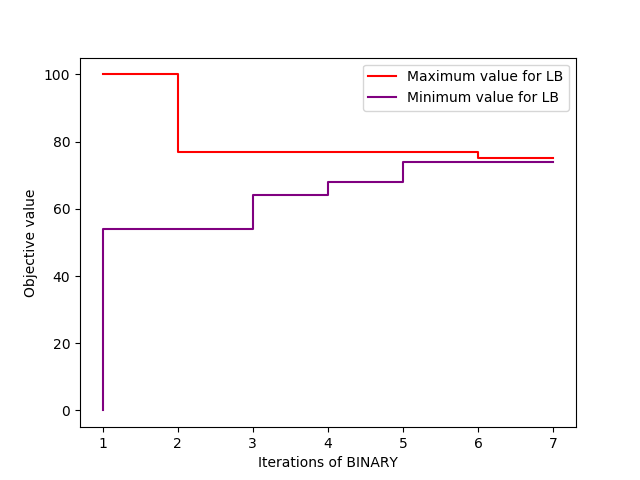
\includegraphics[width=0.72\textwidth]{../imgs/binary_bounds.png}
        \caption{Search space of BINARY algorithm for finding the
        lower bound \\ on easy/instance10\_1\_1.dat}
    \end{center}
\end{figure}

BINARY requires 6 iterations in average to converge while DB3 requires 6 iterations in average.
This seemingly confirms the $\mathcal{O}\left( \log_2 K \right)$ complexity of the bisection search
and the $\mathcal{O}(\log_3 T)$ complexity of DB3.

\begin{figure}[h!]
    \begin{center}
        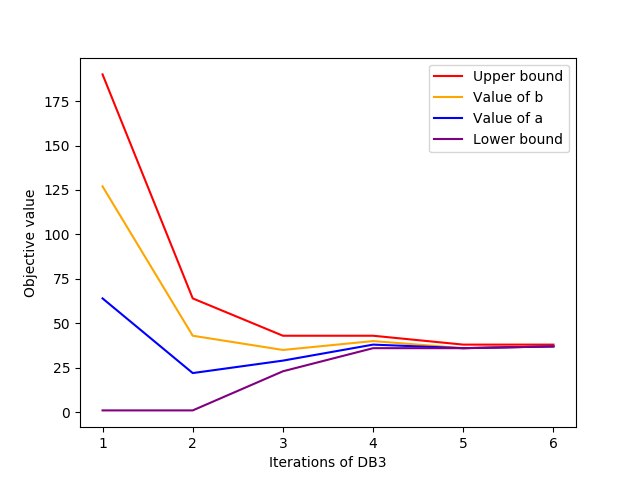
\includegraphics[width=0.72\textwidth]{../imgs/db3_bounds.png}
        \caption{Evolution of lower and upper bounds using DB3 \\
        algorithm on instance hard/instance9.dat}
    \end{center}
\end{figure}
